\chapter{Complex Kinetics: Chains, Enzymes and Oscillations}\label{ch:b3:complex-kinetics}

A beaker of a stirred solution turns colourless, then amber, then blue, then
colourless again, and keeps doing so for many minutes; poured into a dish, the
same mixture draws spirals that rotate and travel. When Boris Belousov
described such a reaction in 1951, his manuscript was rejected: a chemical
system, the referee thought, cannot run back and forth, since it must go
downhill towards equilibrium. It does go downhill; it simply does not go
straight. This chapter treats mechanisms with many steps whose intermediates
are regenerated: \omterm{def:b3:complex-kinetics:chain}{chain reactions} and explosions, molecules that need
collisions to fall apart alone, \omterm{def:b3:complex-kinetics:enzyme}{enzymes}, and the \omterm{def:b3:complex-kinetics:oscillating}{oscillating reactions}, with
the methods that follow reactions too fast to mix by hand.

\begin{recall}
The Year 1 volume defined a reaction mechanism as a sequence of elementary
steps, the rate-determining step, the pre-equilibrium and steady-state
approximations, and catalysts. The Year 2 volume named the steps of a radical
chain (initiation, propagation, termination), radical initiators and the
kinetic chain length of a polymerisation, and fitted least-squares lines.
\Cref{ch:b3:rate-theories} gave \omterm{def:b3:rate-theories:tst}{transition-state theory} and the diffusion limit
of about \qty{e10}{L.mol^{-1}.s^{-1}}.
\end{recall}

\section{Chain reactions}

\begin{definition}[Chain reaction, chain carrier]\label{def:b3:complex-kinetics:chain}
A \emph{chain reaction}\index{chain reaction} is a reaction in which reactive
intermediates, the \emph{chain carriers}\index{chain carrier}, are regenerated by
a cycle of propagation steps, so that one initiation event converts many
reactant molecules.
\end{definition}

Bodenstein measured in 1906 the rate of $\ce{H2 + Br2 -> 2 HBr}$ and found a law that
no single step could produce: the rate grows as $[\ce{Br2}]^{1/2}$ and falls as HBr
accumulates. The mechanism was written down in 1919:
\begin{center}
\begin{tabular}{lll}
initiation & $\ce{Br2 -> 2 Br}$ & $k_1$ \\
propagation & $\ce{Br + H2 -> HBr + H}$ & $k_2$ \\
propagation & $\ce{H + Br2 -> HBr + Br}$ & $k_3$ \\
inhibition & $\ce{H + HBr -> H2 + Br}$ & $k_4$ \\
termination & $\ce{2 Br -> Br2}$ & $k_{-1}$
\end{tabular}
\end{center}
(collisions with a third body M that carry energy in and out of the
initiation and termination steps are left implicit).

\begin{theorem}[The hydrogen--bromine rate law]\label{thm:b3:complex-kinetics:hbr}
With the steady-state approximation for Br and H, the rate $v = \frac12\,\dd[\ce{HBr}]/\dd t$
of the mechanism is
\[
  v = \frac{k[\ce{H2}][\ce{Br2}]^{1/2}}{1 + k'[\ce{HBr}]/[\ce{Br2}]},
  \qquad k = k_2\Bigl(\frac{k_1}{k_{-1}}\Bigr)^{1/2},\ k' = \frac{k_4}{k_3}.
\]
\end{theorem}

\begin{proof}
Steady state for H: $k_2[\ce{Br}][\ce{H2}] = k_3[\ce{H}][\ce{Br2}] + k_4[\ce{H}][\ce{HBr}]$. Steady state for Br:
$2k_1[\ce{Br2}] - k_2[\ce{Br}][\ce{H2}] + k_3[\ce{H}][\ce{Br2}] + k_4[\ce{H}][\ce{HBr}] - 2k_{-1}[\ce{Br}]^2 = 0$. Adding the two
equations, the propagation terms cancel: $k_1[\ce{Br2}] = k_{-1}[\ce{Br}]^2$, so $[\ce{Br}] =
(k_1/k_{-1})^{1/2}[\ce{Br2}]^{1/2}$. Then $[\ce{H}] = k_2[\ce{Br}][\ce{H2}]/(k_3[\ce{Br2}] + k_4[\ce{HBr}])$ and
\[
  \frac{\dd[\ce{HBr}]}{\dd t} = k_2[\ce{Br}][\ce{H2}] + k_3[\ce{H}][\ce{Br2}] - k_4[\ce{H}][\ce{HBr}] = 2k_3[\ce{H}][\ce{Br2}]
  = \frac{2k_2[\ce{Br}][\ce{H2}]}{1 + (k_4/k_3)[\ce{HBr}]/[\ce{Br2}]},
\]
using the first equation; substituting $[\ce{Br}]$ gives the result.
\end{proof}

\begin{omfigure}
\begin{tikzpicture}[font=\small, >=Stealth]
  \node[draw, circle, minimum size=9mm, omDef, thick] (br) at (0,0) {Br};
  \node[draw, circle, minimum size=9mm, omThm, thick] (h) at (4,0) {H};
  \draw[->, thick] (br) to[bend left=35] node[midway, above, align=center] {$+\,\ce{H2}$\\ $\to$ HBr} (h);
  \draw[->, thick] (h) to[bend left=35] node[midway, below, align=center] {$+\,\ce{Br2}$\\ $\to$ HBr} (br);
  \draw[->, thick, black!60] (-2.4,0) -- (br) node[pos=0, left, align=right] {initiation\\ $\ce{Br2 -> 2 Br}$};
  \draw[->, thick, black!60] (br) -- (0,-2.0) node[below, align=center] {termination\\ $\ce{2 Br -> Br2}$};
  \draw[->, thick, black!60, dashed] (h) -- (6.2,-1.2) node[below, align=center] {inhibition\\ $\ce{H + HBr -> H2 + Br}$};
\end{tikzpicture}

{\small The propagation cycle of the hydrogen--bromine chain: each turn consumes
one \ce{H2} and one \ce{Br2}, makes two HBr and gives back the bromine atom that
started it. Initiation feeds the cycle with carriers, termination removes them;
the inhibition step turns an H atom back into Br at the cost of an HBr already
made.}
\end{omfigure}

\begin{omfigure}
\begin{tikzpicture}
\begin{axis}[name=ca, width=0.47\linewidth, height=5.2cm, xmin=0, xmax=800, ymin=0, ymax=1,
  axis lines=left, xlabel={$t$ (reduced)}, ylabel={$[\ce{HBr}]/2[\ce{H2}]_0$},
  tick label style={font=\small}, label style={font=\small}]
\addplot[omDef, thick] table[x=t, y expr=\thisrow{HBr}/2] {figdata/out/bachelor-3-chain-kinetics.dat};
\end{axis}
\begin{axis}[at={(ca.east)}, anchor=west, xshift=1.4cm, width=0.47\linewidth, height=5.2cm,
  xmin=0, xmax=60, ymin=0, ymax=2.2, axis lines=left, xlabel={$t$ (reduced)},
  ylabel={rate $\times 10^3$}, tick label style={font=\small}, label style={font=\small},
  legend style={font=\scriptsize, draw=none, at={(0.97,0.03)}, anchor=south east},
  legend cell align=left]
\addplot[omDef, thick] table[x=t, y expr=1000*\thisrow{v}] {figdata/out/bachelor-3-chain-kinetics.dat};
\addplot[omThm, thick, dashed] table[x=t, y expr=1000*\thisrow{vss}] {figdata/out/bachelor-3-chain-kinetics.dat};
\legend{full mechanism, steady-state law}
\end{axis}
\end{tikzpicture}

{\small The hydrogen--bromine mechanism integrated step by step (model rate
constants, reduced units, $k' = 0.1$): conversion against time (left), and the rate
$\frac12\dd[\ce{HBr}]/\dd t$ of the full mechanism compared with the steady-state law (right).
After an induction period, during which the bromine atoms build up, the two
coincide to better than 1\,\%.}
\end{omfigure}

\begin{method}[The rate law of a chain mechanism]\label{met:b3:complex-kinetics:steady-state-chain}
\begin{enumerate}
  \item Write a steady-state equation for each \omterm{def:b3:complex-kinetics:chain}{chain carrier}.
  \item Add them: the propagation steps, which only exchange one carrier for
        another, cancel, leaving initiation equal to termination; this gives the
        carrier concentration.
  \item Use one carrier's equation to express the other carriers.
  \item Write the rate of formation of a product from the propagation steps.
\end{enumerate}
\end{method}

The number of propagation cycles per initiation event, here $v/k_1[\ce{Br2}]$, is the
kinetic chain length of the Year 2 volume; for the hydrogen--bromine reaction
it is of the order of $10^3$ to $10^6$ depending on the conditions. Inhibition by
the product explains why the rate falls faster than the reactants are consumed.

\section{Branching chains and explosions}

\begin{definition}[Chain branching, explosion limits]\label{def:b3:complex-kinetics:branching}
\emph{Chain branching}\index{chain branching} is a propagation step that produces
more \omterm{def:b3:complex-kinetics:chain}{chain carriers} than it consumes, such as $\ce{H + O2 -> OH + O}$, which turns one
carrier into two. The \emph{explosion limits}\index{explosion limits} of a mixture
are the pressures, at a given temperature, at which its slow reaction turns
into an explosion.
\end{definition}

\begin{proposition}[Branching criterion]\label{prop:b3:complex-kinetics:branching}
Let carriers be created at the rate $v_i$, multiply by branching with the rate
constant $f$ and disappear by termination with the rate constant $g$:
$\dd n/\dd t = v_i + (f - g)n$. If $f < g$, $n$ tends to the steady value $v_i/(g - f)$; if
$f > g$, $n$ grows exponentially and the reaction explodes.
\end{proposition}

\begin{proof}
The linear equation has the solution $n(t) = \frac{v_i}{g - f}\bigl(1 - \eu^{-(g - f)t}\bigr)$, which
tends to $v_i/(g - f)$ when $g > f$; when $f > g$ the exponent is positive and $n$
grows as $\eu^{(f - g)t}$ without bound (until the reactants run out).
\end{proof}

For hydrogen--oxygen mixtures at a few hundred degrees, $f$ grows with the
pressure (it is proportional to $[\ce{O2}]$), termination at the walls of the
vessel is fast at low pressure (the radicals diffuse there easily), and
termination by three-body collisions ($\ce{H + O2 + M -> HO2 + M}$) grows as the square
of the pressure. Branching wins between a first limit, set by the walls, and a
second limit, set by three-body termination; at still higher pressure a third
limit appears where the heat released can no longer escape. The last is a
thermal explosion, driven by the exponential growth of the rate with
temperature rather than by branching; most industrial explosions are of that
kind.

\section{Unimolecular reactions}

A molecule such as cyclopropane isomerises alone, with first-order kinetics at
ordinary pressures; yet at low pressure the rate constant falls. The energy
needed comes from collisions.

\begin{definition}[Lindemann mechanism, fall-off region]\label{def:b3:complex-kinetics:lindemann}
The \emph{Lindemann mechanism}\index{Lindemann mechanism} of a unimolecular
reaction is the sequence $\mathrm{A + M \rightleftharpoons A^* + M}$ ($k_1$, $k_{-1}$), activation and
deactivation by collision with any molecule M, followed by $\mathrm{A^* \to P}$ ($k_2$). The
\emph{fall-off region}\index{fall-off region} is the range of pressures where the
observed first-order rate constant falls from its high-pressure value towards
second-order behaviour.
\end{definition}

\begin{theorem}[Lindemann rate constant]\label{thm:b3:complex-kinetics:lindemann}
With the steady-state approximation for $\mathrm{A^*}$, $v = k_{\mathrm{uni}}[\mathrm A]$ with
\[
  k_{\mathrm{uni}} = \frac{k_1k_2[\mathrm M]}{k_{-1}[\mathrm M] + k_2},
\]
which tends to $k_\infty = k_1k_2/k_{-1}$ at high pressure (first order) and to $k_1[\mathrm M]$ at
low pressure (second order); it is $k_\infty/2$ at $[\mathrm M]_{1/2} = k_2/k_{-1}$.
\end{theorem}

\begin{proof}
$\dd[\mathrm{A^*}]/\dd t = k_1[\mathrm A][\mathrm M] - k_{-1}[\mathrm{A^*}][\mathrm M] - k_2[\mathrm{A^*}] = 0$ gives $[\mathrm{A^*}] =
k_1[\mathrm A][\mathrm M]/(k_{-1}[\mathrm M] + k_2)$ and $v = k_2[\mathrm{A^*}]$. If $k_{-1}[\mathrm M] \gg k_2$, deactivation
outruns reaction and $\mathrm{A^*}$ is in pre-equilibrium: $k_{\mathrm{uni}} \to k_1k_2/k_{-1}$. If $k_{-1}[\mathrm M]
\ll k_2$, every activated molecule reacts and activation is rate-determining:
$k_{\mathrm{uni}} \to k_1[\mathrm M]$.
\end{proof}

\begin{omfigure}
\begin{tikzpicture}
\begin{axis}[width=0.66\linewidth, height=5.4cm, xmode=log, ymode=log, xmin=1e-10, xmax=1e-2,
  ymin=1e-8, ymax=4e-3, axis lines=left, xlabel={$[\mathrm M]$ / \unit{mol.L^{-1}}},
  ylabel={$k_{\mathrm{uni}}$ / \unit{s^{-1}}}, tick label style={font=\small}, label style={font=\small}]
\addplot[black!40, dashed] table[x=M, y=low] {figdata/out/bachelor-3-lindemann.dat};
\addplot[black!40, dashed] table[x=M, y=high] {figdata/out/bachelor-3-lindemann.dat};
\addplot[omDef, very thick] table[x=M, y=k] {figdata/out/bachelor-3-lindemann.dat};
\node[font=\scriptsize, anchor=south, rotate=39] at (axis cs:4e-9,2.5e-5) {$k_1[\mathrm M]$};
\node[font=\scriptsize, anchor=south] at (axis cs:3e-4,1e-3) {$k_\infty$};
\draw[black!50, densely dotted] (axis cs:1e-6,1e-8) -- (axis cs:1e-6,5e-4);
\node[font=\scriptsize, anchor=north west] at (axis cs:1.2e-6,2e-7) {$[\mathrm M]_{1/2}$};
\end{axis}
\end{tikzpicture}

{\small The Lindemann fall-off curve (model constants): first order with the
limiting constant $k_\infty$ at high pressure, second order ($k_1[\mathrm M]$) at low pressure,
and half of $k_\infty$ at $[\mathrm M]_{1/2} = k_2/k_{-1}$. Real fall-off curves are broader: the rate
constant $k_2$ of an energised molecule grows with its energy.}
\end{omfigure}

\section{Enzyme kinetics}

\begin{definition}[Enzyme, active site, enzyme--substrate complex]\label{def:b3:complex-kinetics:enzyme}
An \emph{enzyme}\index{enzyme} is a biological catalyst, almost always a protein,
that speeds up a specific reaction of its substrate. The \emph{active
site}\index{active site} is the pocket of the enzyme where the substrate binds
and reacts; the bound species is the \emph{enzyme--substrate
complex}\index{enzyme--substrate complex} ES.
\end{definition}

\begin{definition}[Michaelis constant, maximum rate, catalytic and specificity constants]\label{def:b3:complex-kinetics:michaelis}
For the mechanism $\mathrm{E + S \rightleftharpoons ES \to E + P}$ ($k_1$, $k_{-1}$, $k_2$) at total \omterm{def:b3:complex-kinetics:enzyme}{enzyme} concentration
$[\mathrm E]_0$, the \emph{catalytic constant}\index{catalytic constant} is $k_{\mathrm{cat}} = k_2$, the
\emph{maximum rate}\index{maximum rate} is $V_{\max} = k_{\mathrm{cat}}[\mathrm E]_0$, the \emph{Michaelis
constant}\index{Michaelis constant} is $K_M = (k_{-1} + k_2)/k_1$, and the \emph{specificity
constant}\index{specificity constant} is $k_{\mathrm{cat}}/K_M$.
\end{definition}

\begin{theorem}[Michaelis--Menten equation]\label{thm:b3:complex-kinetics:michaelis-menten}
When $[\mathrm S] \gg [\mathrm E]_0$ and ES is in a steady state, the initial rate of formation of
the product is
\[
  v = \frac{V_{\max}[\mathrm S]}{K_M + [\mathrm S]} .
\]
This statement is the \emph{Michaelis--Menten equation}\index{Michaelis--Menten
equation}.
\end{theorem}

\begin{proof}
Steady state: $k_1[\mathrm E][\mathrm S] = (k_{-1} + k_2)[\mathrm{ES}]$, and $[\mathrm E] = [\mathrm E]_0 - [\mathrm{ES}]$ (the free
substrate is practically all the substrate since $[\mathrm S] \gg [\mathrm E]_0$). Hence $[\mathrm{ES}]
= [\mathrm E]_0[\mathrm S]/(K_M + [\mathrm S])$ and $v = k_2[\mathrm{ES}]$.
\end{proof}

\begin{remark}
Michaelis and Menten (1913) assumed instead a rapid pre-equilibrium of E, S and
ES; the same equation follows with $K_M$ replaced by the dissociation constant
$k_{-1}/k_1$, the limit of $K_M$ when $k_2 \ll k_{-1}$. The \omterm{def:b3:complex-kinetics:michaelis}{catalytic constant} is what
biochemists call the turnover number of the \omterm{def:b3:complex-kinetics:enzyme}{enzyme}: the number of substrate
molecules one \omterm{def:b3:complex-kinetics:enzyme}{active site} converts per second when saturated.
\end{remark}

At $[\mathrm S] = K_M$ the rate is $V_{\max}/2$; at $[\mathrm S] \ll K_M$ it is $(k_{\mathrm{cat}}/K_M)[\mathrm E]_0[\mathrm S]$: the
\omterm{def:b3:complex-kinetics:michaelis}{specificity constant} is the second-order rate constant of the free \omterm{def:b3:complex-kinetics:enzyme}{enzyme} with
its substrate, and it cannot exceed the rate at which they meet, the
diffusion limit of \cref{ch:b3:rate-theories}. A few \omterm{def:b3:complex-kinetics:enzyme}{enzymes} come close; the
``average'' \omterm{def:b3:complex-kinetics:enzyme}{enzyme}, in a survey of several thousand, has $k_{\mathrm{cat}}/K_M$ of about
$10^5$~\unit{L.mol^{-1}.s^{-1}}, some four orders of magnitude below.

\begin{proposition}[Lineweaver--Burk form]\label{prop:b3:complex-kinetics:lineweaver}
The \omterm{thm:b3:complex-kinetics:michaelis-menten}{Michaelis--Menten equation} is equivalent to
\[
  \frac1v = \frac{1}{V_{\max}} + \frac{K_M}{V_{\max}}\,\frac{1}{[\mathrm S]},
\]
a straight line of $1/v$ against $1/[\mathrm S]$ with intercept $1/V_{\max}$, slope $K_M/V_{\max}$, and
intercept $-1/K_M$ on the $1/[\mathrm S]$ axis.
\end{proposition}

\begin{proof}
Invert: $1/v = (K_M + [\mathrm S])/(V_{\max}[\mathrm S])$. At $1/v = 0$, $1/[\mathrm S] = -1/K_M$.
\end{proof}

\begin{method}[$K_M$ and $V_{\max}$ by nonlinear least squares]\label{met:b3:complex-kinetics:mm-fit}
\begin{enumerate}
  \item Measure initial rates at substrate concentrations spread from about
        $K_M/5$ to $10K_M$.
  \item Fit $v = V_{\max}[\mathrm S]/(K_M + [\mathrm S])$ directly, by minimising $\sum(v_i - v(\mathrm S_i))^2$ (iteratively,
        starting from the values of a Lineweaver--Burk line); the standard
        errors come from the residuals and the sensitivity of $v$ to each
        parameter.
  \item Use the Lineweaver--Burk plot only to see the pattern: inverting small
        rates magnifies their errors, so the least-squares line through $1/v$
        is dominated by the least precise points, and its parameters are
        biased.
\end{enumerate}
\end{method}

\begin{definition}[Inhibition]\label{def:b3:complex-kinetics:inhibition}
An inhibitor I binds the \omterm{def:b3:complex-kinetics:enzyme}{enzyme} reversibly. In \emph{competitive
inhibition}\index{competitive inhibition} it binds only the free \omterm{def:b3:complex-kinetics:enzyme}{enzyme}, at the
\omterm{def:b3:complex-kinetics:enzyme}{active site}, with the \emph{inhibition constant}\index{inhibition constant} $K_i$
(dissociation constant of EI); in \emph{uncompetitive inhibition}\index{uncompetitive
inhibition} it binds only ES, with the constant $K_i'$; in \emph{mixed
inhibition}\index{mixed inhibition} it binds both.
\end{definition}

\begin{proposition}[Inhibited rate laws]\label{prop:b3:complex-kinetics:inhibition-laws}
With $\alpha = 1 + [\mathrm I]/K_i$ and $\alpha' = 1 + [\mathrm I]/K_i'$, the rate keeps the
Michaelis--Menten form $v = V^{\mathrm{app}}[\mathrm S]/(K_M^{\mathrm{app}} + [\mathrm S])$ with: competitive,
$K_M^{\mathrm{app}} = \alpha K_M$, $V^{\mathrm{app}} = V_{\max}$; uncompetitive, $K_M^{\mathrm{app}} = K_M/\alpha'$, $V^{\mathrm{app}} =
V_{\max}/\alpha'$; mixed, $K_M^{\mathrm{app}} = \alpha K_M/\alpha'$, $V^{\mathrm{app}} = V_{\max}/\alpha'$.
\end{proposition}

\begin{proof}
Mixed case (the others are its limits $K_i' \to \infty$ and $K_i \to \infty$): the \omterm{def:b3:complex-kinetics:enzyme}{enzyme} is
shared among E, EI, ES and ESI with $[\mathrm{EI}] = [\mathrm E][\mathrm I]/K_i$, $[\mathrm{ESI}] = [\mathrm{ES}][\mathrm I]/K_i'$
and the steady state $[\mathrm E][\mathrm S] = K_M[\mathrm{ES}]$. So $[\mathrm E]_0 = [\mathrm E]\alpha + [\mathrm{ES}]\alpha' =
[\mathrm{ES}](\alpha K_M/[\mathrm S] + \alpha')$ and $v = k_2[\mathrm{ES}] = V_{\max}[\mathrm S]/(\alpha K_M + \alpha'[\mathrm S])$; dividing numerator
and denominator by $\alpha'$ gives the stated form.
\end{proof}

\begin{method}[Recognising the type of inhibition]\label{met:b3:complex-kinetics:inhibition-type}
\begin{enumerate}
  \item Measure $v([\mathrm S])$ at several inhibitor concentrations and draw the
        Lineweaver--Burk lines.
  \item Lines meeting on the $1/v$ axis (same $V_{\max}$): competitive; a large excess
        of substrate overcomes the inhibitor.
  \item Parallel lines (slope $K_M/V_{\max}$ unchanged): uncompetitive.
  \item Lines meeting to the left of the $1/v$ axis: mixed.
  \item Obtain $K_i$ by fitting the apparent constants against $[\mathrm I]$: for a
        competitive inhibitor $K_M^{\mathrm{app}} = K_M + (K_M/K_i)[\mathrm I]$, a straight line.
\end{enumerate}
\end{method}

\begin{omfigure}
\begin{tikzpicture}
\begin{axis}[name=mv, width=0.47\linewidth, height=5.4cm, xmin=0, xmax=8, ymin=0, ymax=0.55,
  axis lines=left, xlabel={$[\mathrm S]$ / mM}, ylabel={$v$ / \unit{\micro M.s^{-1}}},
  tick label style={font=\small}, label style={font=\small},
  legend style={font=\scriptsize, draw=none, fill=white, fill opacity=0.85, text opacity=1,
  at={(0.97,0.03)}, anchor=south east}, legend cell align=left]
\addplot[black, thick] table[x=S, y=none] {figdata/out/bachelor-3-michaelis-menten-model.dat};
\addplot[omDef, thick] table[x=S, y=comp] {figdata/out/bachelor-3-michaelis-menten-model.dat};
\addplot[omThm, thick] table[x=S, y=uncomp] {figdata/out/bachelor-3-michaelis-menten-model.dat};
\draw[black!40, densely dotted] (axis cs:0,0.25) -- (axis cs:0.8,0.25) -- (axis cs:0.8,0);
\node[font=\scriptsize, anchor=north west] at (axis cs:0.85,0.12) {$K_M$};
\legend{no inhibitor, competitive, uncompetitive}
\end{axis}
\begin{axis}[at={(mv.east)}, anchor=west, xshift=1.5cm, width=0.47\linewidth, height=5.4cm,
  xmin=-2.5, xmax=3.5, ymin=0, ymax=12, axis x line=middle, axis y line=middle,
  tick label style={font=\small}, xtick={-2,-1,1,2,3}]
\node[font=\small, anchor=south east] at (axis cs:3.5,0.3) {$1/[\mathrm S]$};
\node[font=\small, anchor=north west] at (axis cs:0.12,12) {$1/v$};
\addplot[black, thick, domain=-1.25:3.5] {1.6*x + 2};
\addplot[omDef, thick, domain=-0.4167:3.5] {4.8*x + 2};
\addplot[omThm, thick, domain=-2.5:3.5] {1.6*x + 4};
\end{axis}
\end{tikzpicture}

{\small Michaelis--Menten kinetics with $K_M = \qty{0.80}{mM}$ and $V_{\max} = \qty{0.50}{\micro M.s^{-1}}$
(model): no inhibitor (black), a competitive inhibitor at $[\mathrm I] = 2K_i$ (blue,
$K_M$ tripled, same $V_{\max}$) and an uncompetitive one at $[\mathrm I] = K_i'$ (red, $K_M$ and
$V_{\max}$ halved). Right: the Lineweaver--Burk lines; the competitive line meets
the uninhibited one on the $1/v$ axis, the uncompetitive one is parallel to it
($1/[\mathrm S]$ in \unit{mM^{-1}}, $1/v$ in \unit{s.\micro M^{-1}}).}
\end{omfigure}

\section{Autocatalysis, oscillations and fast reactions}

\begin{definition}[Autocatalytic reaction]\label{def:b3:complex-kinetics:autocatalysis}
An \emph{autocatalytic reaction}\index{autocatalytic reaction} is one in which a
product catalyses its own formation, as in $\mathrm{A + X \to 2\,X}$.
\end{definition}

\begin{proposition}[Logistic law]\label{prop:b3:complex-kinetics:logistic}
For $\mathrm{A + X \to 2\,X}$ with rate constant $k$ and initial concentrations $a_0$ and $x_0$,
with $N = a_0 + x_0$,
\[
  x(t) = \frac{N}{1 + (N/x_0 - 1)\eu^{-kNt}},
\]
an S-shaped curve that reaches half its final value at $t_{1/2} = \ln(N/x_0 - 1)/kN$.
\end{proposition}

\begin{proof}
$\dd x/\dd t = kx(N - x)$, since $a = N - x$. Separating, $\frac{\dd x}{x(N - x)} = \frac1N\bigl(\frac1x + \frac{1}{N - x}\bigr)\dd x
= k\,\dd t$, so $\ln\frac{x}{N - x} = kNt + \ln\frac{x_0}{N - x_0}$, which rearranges into the stated form;
$x = N/2$ when $(N/x_0 - 1)\eu^{-kNt} = 1$.
\end{proof}

\begin{definition}[Oscillating reaction, limit cycle]\label{def:b3:complex-kinetics:oscillating}
An \emph{oscillating reaction}\index{oscillating reaction} is one in which the
concentrations of intermediates rise and fall periodically while the overall
reaction proceeds towards equilibrium. A \emph{limit cycle}\index{limit cycle} is
a closed trajectory in the space of concentrations towards which neighbouring
trajectories converge, so that the oscillation has an amplitude independent
of the starting point.
\end{definition}

\begin{theorem}[Lotka--Volterra model]\label{thm:b3:complex-kinetics:lotka-volterra}
For the autocatalytic scheme $\mathrm{A + X \to 2\,X}$, $\mathrm{X + Y \to 2\,Y}$, $\mathrm{Y \to B}$ with A held
constant, the concentrations obey $\dot x = x(a - by)$, $\dot y = y(dx - c)$ with positive
constants, and the quantity
\[
  V = dx - c\ln x + by - a\ln y
\]
is constant along each trajectory: the trajectories are closed curves around
the steady state $(c/d, a/b)$, and the concentrations oscillate with an
amplitude fixed by the starting point.
\end{theorem}

\begin{proof}
$\dot V = (d - c/x)\dot x + (b - a/y)\dot y = (dx - c)(a - by) + (by - a)(dx - c) = 0$. $V$ is a
sum of two convex functions with a single minimum at $(c/d, a/b)$, so its level
curves are closed curves around that point; a trajectory stays on one of
them and, the velocity never vanishing elsewhere, goes round it periodically.
\end{proof}

The Lotka--Volterra oscillations are fragile: every starting point gives its
own orbit, and any perturbation moves the system to another. Real chemical
oscillators have a \omterm{def:b3:complex-kinetics:oscillating}{limit cycle}, which needs a nonlinearity that destabilises
the steady state.

\begin{proposition}[Instability of the Brusselator]\label{prop:b3:complex-kinetics:hopf}
The model $\dot X = A - (B + 1)X + X^2Y$, $\dot Y = BX - X^2Y$ (reduced concentrations,
$A$ and $B$ held constant) has the single steady state $(A, B/A)$, which is
stable if $B < 1 + A^2$ and unstable if $B > 1 + A^2$; the system then settles on a
\omterm{def:b3:complex-kinetics:oscillating}{limit cycle}.
\end{proposition}

\begin{proof}
Setting both derivatives to zero: $BX = X^2Y$ gives $XY = B$, and then $A - X = 0$. The
Jacobian matrix at $(A, B/A)$ is
\[
  \begin{pmatrix} -(B + 1) + 2XY & X^2 \\ B - 2XY & -X^2 \end{pmatrix}
  = \begin{pmatrix} B - 1 & A^2 \\ -B & -A^2 \end{pmatrix},
\]
with trace $B - 1 - A^2$ and determinant $A^2 > 0$. Small deviations evolve as
$\eu^{\lambda t}$ with $\lambda$ the \omterm{def:b3:quantum-model-systems:operator}{eigenvalues}, whose product is the determinant (positive)
and whose sum is the trace: both have negative real parts when the trace is
negative, positive real parts when it is positive. The existence of the \omterm{def:b3:complex-kinetics:oscillating}{limit
cycle} for $B > 1 + A^2$ (the trajectories being confined to a bounded region) is
admitted.
\end{proof}

\begin{method}[The linear stability of a steady state]\label{met:b3:complex-kinetics:stability}
\begin{enumerate}
  \item Find the steady state by setting all time derivatives to zero.
  \item Compute the Jacobian matrix of partial derivatives of the rates there.
  \item For two variables: stable if the trace is negative and the determinant
        positive; an unstable state with complex \omterm{def:b3:quantum-model-systems:operator}{eigenvalues}
        ($\mathrm{tr}^2 < 4\det$) gives growing oscillations, a candidate \omterm{def:b3:complex-kinetics:oscillating}{limit cycle}.
\end{enumerate}
\end{method}

\begin{omfigure}
\begin{tikzpicture}
\begin{axis}[name=bs, width=0.62\linewidth, height=4.6cm, xmin=0, xmax=40, ymin=0, ymax=5.2,
  axis lines=left, xlabel={$t$ (reduced)}, ylabel={concentration},
  tick label style={font=\small}, label style={font=\small},
  legend style={font=\scriptsize, draw=none, at={(1.03,0.98)}, anchor=north west}]
\addplot[omDef, thick] table[x=t, y=X] {figdata/out/bachelor-3-oscillations-series.dat};
\addplot[omThm, thick] table[x=t, y=Y] {figdata/out/bachelor-3-oscillations-series.dat};
\legend{$X$, $Y$}
\end{axis}
\begin{axis}[name=ph, at={(bs.below south west)}, anchor=north west, yshift=-0.6cm,
  width=0.42\linewidth, height=5.0cm, xmin=0, xmax=4.8, ymin=0, ymax=5.6, axis lines=left,
  xlabel={$X$}, ylabel={$Y$}, tick label style={font=\small}, label style={font=\small},
  title={\small Brusselator}]
\addplot[omDef, thin] table[x=X, y=Y] {figdata/out/bachelor-3-oscillations-inner.dat};
\addplot[omThm, thin] table[x=X, y=Y] {figdata/out/bachelor-3-oscillations-outer.dat};
\addplot[only marks, mark=*, mark size=1.5pt] coordinates {(1,3)};
\end{axis}
\begin{axis}[at={(ph.east)}, anchor=west, xshift=1.3cm, width=0.42\linewidth, height=5.0cm,
  xmin=0, xmax=3.2, ymin=0, ymax=3.2, axis lines=left, xlabel={$x$}, ylabel={$y$},
  tick label style={font=\small}, label style={font=\small}, title={\small Lotka--Volterra}]
\addplot[black!70, thick] table[x=x, y=y] {figdata/out/bachelor-3-oscillations-lv1.dat};
\addplot[omDef, thick] table[x=x, y=y] {figdata/out/bachelor-3-oscillations-lv2.dat};
\addplot[omThm, thick] table[x=x, y=y] {figdata/out/bachelor-3-oscillations-lv3.dat};
\addplot[only marks, mark=*, mark size=1.5pt] coordinates {(1,1)};
\end{axis}
\end{tikzpicture}

{\small Top: the Brusselator ($A = 1$, $B = 3 > 1 + A^2$) settles into sustained
oscillations of period 7.2 (reduced time). Bottom left: two trajectories, one
starting near the unstable steady state (dot) and one far outside, wind onto
the same \omterm{def:b3:complex-kinetics:oscillating}{limit cycle}. Bottom right: Lotka--Volterra orbits, each fixed by its
starting point, around the steady state (dot).}
\end{omfigure}

The Belousov--Zhabotinsky reaction, the oxidation of malonic acid by bromate
catalysed by cerium or by a ferroin indicator, runs through such a cycle: an
autocatalytic production of \ce{HBrO2} switches on when bromide falls below a
threshold, oxidises the catalyst (the colour change), and is switched off when
the oxidised catalyst regenerates bromide. Unstirred, in a thin layer, the
oscillation propagates as waves.

\begin{omfigure}
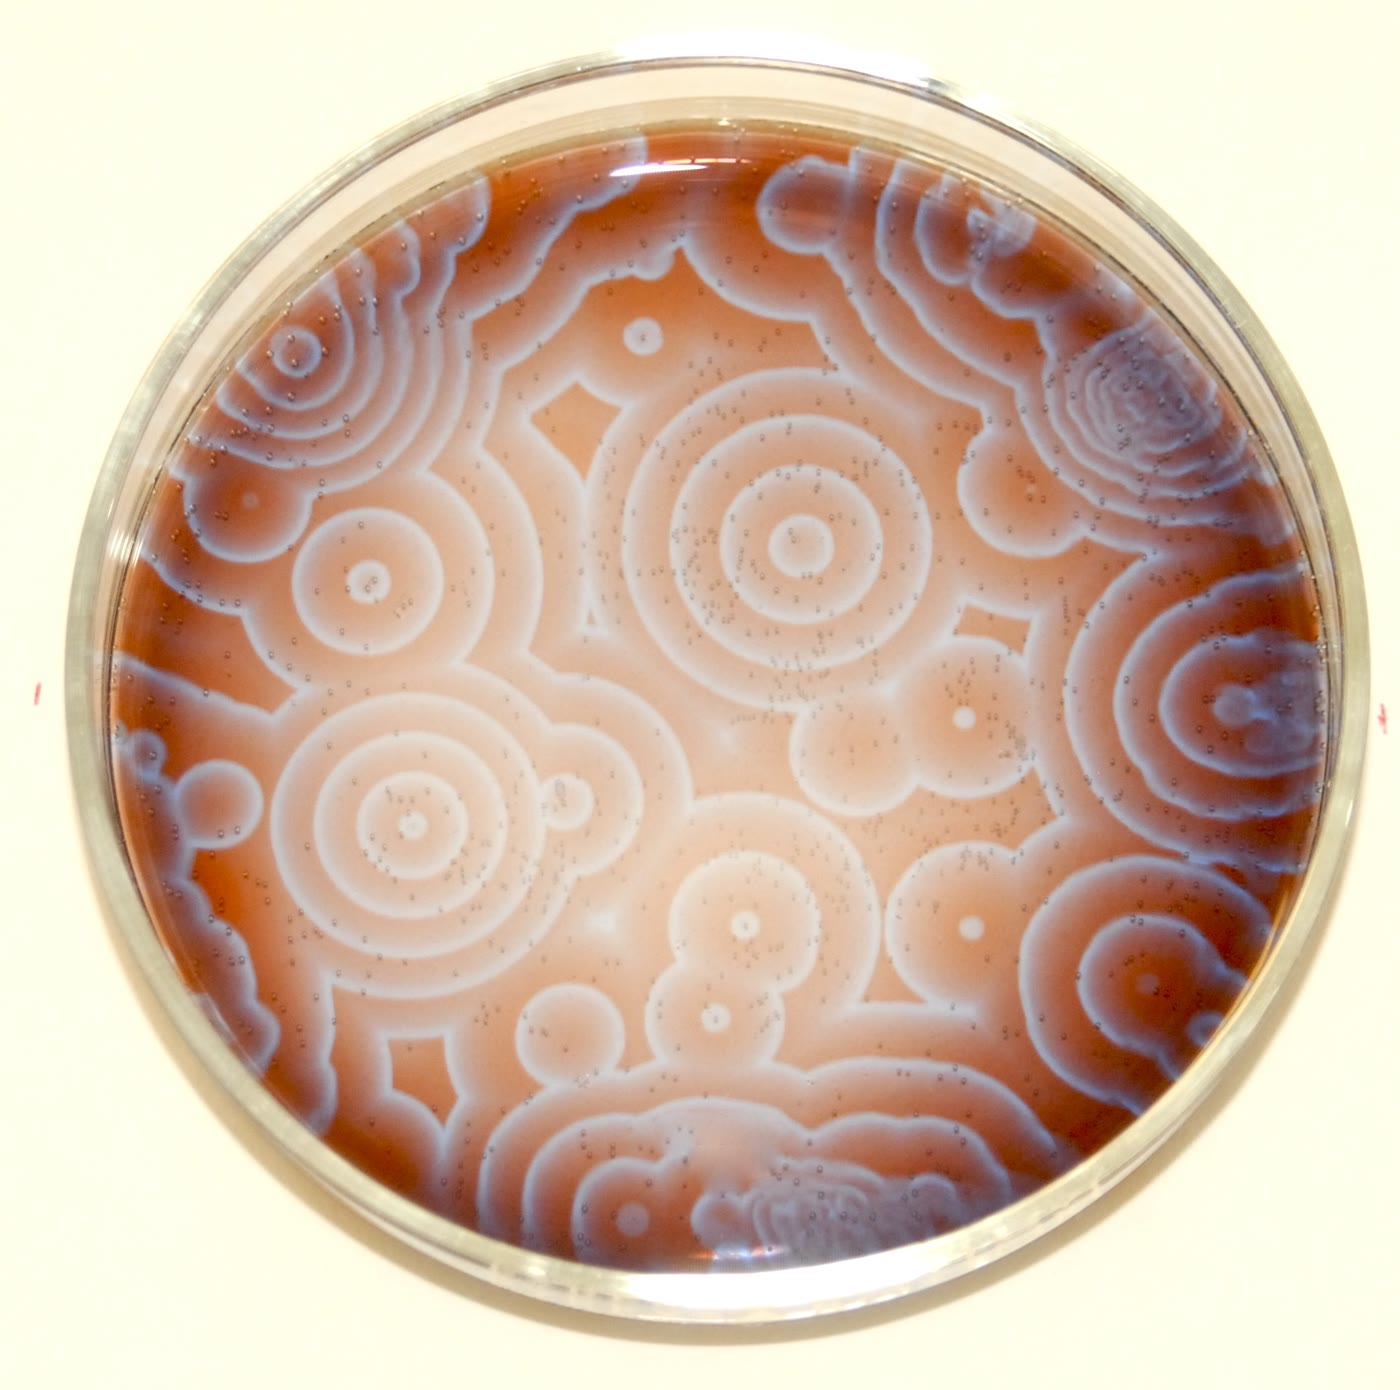
\includegraphics[width=0.48\linewidth]{images/book4/bz-reaction.jpg}

{\small Spiral waves of the Belousov--Zhabotinsky reaction in a thin layer of
solution: each blue front is a wave of oxidation of the catalyst, which
travels into the reduced (red) medium and cannot re-enter the region it just
left.}
\end{omfigure}

\begin{definition}[Relaxation method, chemical relaxation time]\label{def:b3:complex-kinetics:relaxation}
A \emph{relaxation method}\index{relaxation method} perturbs a system at
equilibrium suddenly (by a jump of temperature, pressure or electric field)
and follows its return to the new equilibrium. For a small perturbation the
deviation decays exponentially, with the \emph{chemical relaxation
time}\index{chemical relaxation time} $\tau$.
\end{definition}

\begin{proposition}[Relaxation time of an association]\label{prop:b3:complex-kinetics:relaxation-time}
For $\mathrm{A + B \rightleftharpoons C}$ ($k_1$, $k_{-1}$), after a small perturbation,
\[
  \frac1\tau = k_1([\mathrm A]_e + [\mathrm B]_e) + k_{-1} .
\]
\end{proposition}

\begin{proof}
Write $[\mathrm C] = [\mathrm C]_e + x$, $[\mathrm A] = [\mathrm A]_e - x$, $[\mathrm B] = [\mathrm B]_e - x$. Then $\dot x =
k_1([\mathrm A]_e - x)([\mathrm B]_e - x) - k_{-1}([\mathrm C]_e + x)$; the terms without $x$ cancel at
equilibrium, and dropping $x^2$: $\dot x = -[k_1([\mathrm A]_e + [\mathrm B]_e) + k_{-1}]x$.
\end{proof}

Measuring $\tau$ at several concentrations gives a line of $1/\tau$ against $[\mathrm A]_e +
[\mathrm B]_e$ whose slope is $k_1$ and intercept $k_{-1}$: both constants from experiments
on a system that never leaves equilibrium by more than a few per cent. Manfred
Eigen measured in this way the fastest reactions in solution, among them the
neutralisation of \ce{H3O+} by \ce{OH-}.

\begin{omfigure}
\begin{tikzpicture}
\begin{axis}[width=0.62\linewidth, height=5.0cm, xmin=0, xmax=780, ymin=0, ymax=1.05,
  axis lines=left, xlabel={$t$ / \unit{\micro s}}, ylabel={$([\mathrm C] - [\mathrm C]_e)/([\mathrm C]_0 - [\mathrm C]_e)$},
  tick label style={font=\small}, label style={font=\small},
  legend style={font=\scriptsize, draw=none, at={(0.97,0.97)}, anchor=north east},
  legend cell align=left]
\addplot[omDef, very thick] table[x=t_us, y=dC] {figdata/out/bachelor-3-chemical-relaxation.dat};
\addplot[omThm, thick, dashed] table[x=t_us, y=exp] {figdata/out/bachelor-3-chemical-relaxation.dat};
\legend{full rate equation, {$\eu^{-t/\tau}$, $\tau = \qty{156}{\micro s}$}}
\draw[black!40, densely dotted] (axis cs:156,0) -- (axis cs:156,0.368) -- (axis cs:0,0.368);
\end{axis}
\end{tikzpicture}

{\small Relaxation of $\mathrm{A + B \rightleftharpoons C}$ after a temperature jump that lowered its
equilibrium constant by 5\,\% (model: $k_1 = \qty{1.0e8}{L.mol^{-1}.s^{-1}}$, $k_{-1} = \qty{1.0e3}{s^{-1}}$,
\qty{1.0e-4}{mol/L} of A and B in all): the full rate equation and the exponential with
$1/\tau = k_1([\mathrm A]_e + [\mathrm B]_e) + k_{-1}$ coincide.}
\end{omfigure}

\begin{definition}[Stopped flow, flash photolysis]\label{def:b3:complex-kinetics:fast}
The \emph{stopped-flow method}\index{stopped-flow method} mixes two reactant
solutions in about a millisecond by driving them through a mixer into an
observation cell, then stops the flow and records the absorbance or
\omterm{def:b3:electronic-spectroscopy:luminescence}{fluorescence}. \emph{Flash photolysis}\index{flash photolysis} creates a reactive
species by a short intense light pulse and follows its reactions with a
second, delayed light beam.
\end{definition}

\begin{omfigure}
\begin{tikzpicture}[font=\small, >=Stealth]
  % two drive syringes
  \foreach \y/\lab in {1.1/A, -0.1/B}{
    \draw[thick] (0,\y) rectangle (2.2,\y+0.6);
    \fill[omDef!25] (0.6,\y+0.05) rectangle (2.15,\y+0.55);
    \draw[thick] (0.6,\y) -- (0.6,\y+0.6);
    \draw[thick] (-0.6,\y+0.3) -- (0.6,\y+0.3);
    \node at (1.4,\y+0.3) {\lab};
    \draw[thick] (2.2,\y+0.3) -- (2.8,\y+0.3);}
  \draw[thick] (2.8,1.4) -- (3.2,0.8) (2.8,0.2) -- (3.2,0.8);
  \node[draw, thick, circle, minimum size=5mm, fill=white] (mx) at (3.4,0.8) {};
  \node[font=\scriptsize, anchor=north] at (3.4,0.5) {mixer};
  \draw[thick] (mx.east) -- (4.4,0.8);
  \draw[thick, fill=omThm!15] (4.4,0.55) rectangle (5.4,1.05);
  \node[font=\scriptsize, anchor=north west, align=left] at (5.0,0.5) {observation\\ cell};
  \draw[->, omThm, thick] (4.9,2.0) -- (4.9,1.1) node[pos=0, above, font=\scriptsize] {light};
  \draw[->, omThm, thick] (4.9,0.5) -- (4.9,-0.4) node[below, font=\scriptsize] {detector};
  \draw[thick] (5.4,0.8) -- (6.2,0.8);
  \draw[thick] (6.2,0.5) rectangle (7.6,1.1);
  \draw[thick] (7.0,0.5) -- (7.0,1.1);
  \draw[thick] (7.0,0.8) -- (7.9,0.8);
  \draw[thick] (7.9,0.4) -- (7.9,1.2);
  \node[font=\scriptsize, anchor=south] at (6.9,1.15) {stop syringe};
  \draw[->, black!60] (-1.2,1.4) -- (-0.7,1.4) node[pos=0, left, font=\scriptsize] {drive};
  \draw[->, black!60] (-1.2,0.2) -- (-0.7,0.2);
\end{tikzpicture}

{\small A stopped-flow apparatus. The drive pushes two syringes; the solutions
meet in the mixer and fill the observation cell within about a millisecond;
the plunger of the stop syringe hits a block, the flow stops, and the
detector records the reaction of the freshly mixed solution.}
\end{omfigure}

\begin{omfigure}
\begin{tikzpicture}
\begin{axis}[width=0.62\linewidth, height=5.0cm, xmin=0, xmax=20, ymin=0, ymax=5.5,
  axis lines=left, xlabel={$t$ / ms}, ylabel={$[\mathrm P_1]$ / \unit{\micro M}},
  tick label style={font=\small}, label style={font=\small}]
\addplot[omDef, very thick] table[x=t_ms, y=P_uM] {figdata/out/bachelor-3-michaelis-menten-burst.dat};
\addplot[black!45, dashed, domain=0:20] {1.28 + 0.2*x};
\draw[->, black!60] (axis cs:4.5,0.7) -- (axis cs:0.25,1.24);
\node[font=\scriptsize, anchor=west] at (axis cs:4.5,0.7) {burst amplitude, \qty{1.28}{\micro M}};
\end{axis}
\end{tikzpicture}

{\small A stopped-flow burst trace (data of the weekend problem): the first
product of a two-step \omterm{def:b3:complex-kinetics:enzyme}{enzyme} appears in a fast burst followed by a straight
line; the dashed line extrapolates the steady state back to $t = 0$.}
\end{omfigure}

\begin{inthelab}[A stopped-flow measurement]
The two syringes are filled with \omterm{def:b3:complex-kinetics:enzyme}{enzyme} and substrate solutions in the same
buffer, thermostated, and fired several times to flush the cell before the
recorded shots; each trace is averaged over five to ten shots. The dead time,
the age of the mixture when observation starts, is measured once with a
reaction of known rate.
\end{inthelab}

\begin{safety}{\ghs[0.8cm]{GHS05}\ghs[0.8cm]{GHS06}\ghs[0.8cm]{GHS09}}
% ledger: ghs4:Br2
Bromine: a volatile, dense red-brown liquid; fatal if inhaled, causes severe
burns, very toxic to aquatic life. Handled only in a fume hood, with gloves
and face protection; a solution of sodium thiosulfate is kept at hand to reduce
spills.
\end{safety}

\begin{history}[Bodenstein and Belousov]
Max Bodenstein and Samuel Lind measured the hydrogen--bromine rate law in
1906; Jens Christiansen, Karl Herzfeld and Michael Polanyi explained it in
1919 with the chain mechanism of this chapter. Boris Belousov, a biochemist in
Moscow, found his \omterm{def:b3:complex-kinetics:oscillating}{oscillating reaction} around 1951 while looking for a
chemical model of a metabolic cycle; his manuscript was rejected, and only a
short abstract appeared in 1959. Anatol Zhabotinsky took up the reaction in
the 1960s and explained it; the full mechanism was worked out in the early
1970s.
\end{history}

\section{Exercises}

\begin{exercise}[$\star$]\label{exo:b3:complex-kinetics:1}
For the chain $\ce{Cl2 -> 2 Cl}$, $\ce{Cl + H2 -> HCl + H}$, $\ce{H + Cl2 -> HCl + Cl}$, $\ce{2 Cl -> Cl2}$,
name each step and the \omterm{def:b3:complex-kinetics:chain}{chain carriers}, and write the overall reaction.
\end{exercise}

\begin{exercise}[$\star$]\label{exo:b3:complex-kinetics:2}
A Lindemann system has $k_2 = \qty{1.0e7}{s^{-1}}$ and $k_{-1} = \qty{1.0e10}{L.mol^{-1}.s^{-1}}$ (data of the
exercise). Compute $[\mathrm M]_{1/2}$ and the corresponding pressure at \qty{750}{K}.
\end{exercise}

\begin{exercise}[$\star$]\label{exo:b3:complex-kinetics:3}
Express $v/V_{\max}$ at $[\mathrm S] = K_M$, $3K_M$ and $9K_M$. What concentration gives 90\,\% of
$V_{\max}$?
\end{exercise}

\begin{exercise}[$\star$]\label{exo:b3:complex-kinetics:4}
% ledger: enz:median.kcatKM, visc:H2O.25C
An \omterm{def:b3:complex-kinetics:enzyme}{enzyme} has $k_{\mathrm{cat}} = \qty{100}{s^{-1}}$ and $K_M = \qty{0.80}{mM}$. Compute its \omterm{def:b3:complex-kinetics:michaelis}{specificity
constant} and compare it with the diffusion limit in water, \qty{7.4e9}{L.mol^{-1}.s^{-1}},
and with the typical $10^5$~\unit{L.mol^{-1}.s^{-1}}.
\end{exercise}

\begin{exercise}[$\star\star$]\label{exo:b3:complex-kinetics:5}
The decomposition $\ce{CH3CHO -> CH4 + CO}$ is proposed to run by: $\ce{CH3CHO -> CH3 +
CHO}$ ($k_1$); $\ce{CH3 + CH3CHO -> CH4 + CH3CO}$ ($k_2$); $\ce{CH3CO -> CH3 + CO}$ ($k_3$);
$\ce{2 CH3 -> C2H6}$ ($k_4$). Show that the rate of formation of methane is
$k_2(k_1/2k_4)^{1/2}[\ce{CH3CHO}]^{3/2}$.
\end{exercise}

\begin{exercise}[$\star\star$]\label{exo:b3:complex-kinetics:6}
Starting from equal concentrations of \ce{H2} and \ce{Br2}, with $k' = 0.10$, by what
factor has the rate fallen when half the bromine is consumed? How much of the
fall is due to inhibition?
\end{exercise}

\begin{exercise}[$\star\star$]\label{exo:b3:complex-kinetics:7}
In a model hydrogen--oxygen mixture (data of the exercise), branching has the
rate constant $f = 1000\,p$, wall termination $6000/p$ and three-body termination
$10\,p^2$, all in \unit{s^{-1}} with $p$ in kPa. Find the pressure range in which the mixture
explodes.
\end{exercise}

\begin{exercise}[$\star\star$]\label{exo:b3:complex-kinetics:8}
Initial rates are $\qty{0.20}{\micro M.s^{-1}}$ at $[\mathrm S] = \qty{0.50}{mM}$ and $\qty{0.40}{\micro M.s^{-1}}$ at
\qty{2.0}{mM}. Find $K_M$ and $V_{\max}$.
\end{exercise}

\begin{exercise}[$\star\star$]\label{exo:b3:complex-kinetics:9}
With \qty{50}{\micro M} of an inhibitor, the Lineweaver--Burk line of an \omterm{def:b3:complex-kinetics:enzyme}{enzyme}
($K_M = \qty{0.80}{mM}$) meets the uninhibited one on the $1/v$ axis and crosses the
$1/[\mathrm S]$ axis at \qty{-0.417}{mM^{-1}}. Identify the type of inhibition and compute $K_i$.
\end{exercise}

\begin{exercise}[$\star\star\star$]\label{exo:b3:complex-kinetics:10}
For $\mathrm{A + X \to 2\,X}$ with $k = \qty{0.50}{L.mol^{-1}.s^{-1}}$, $a_0 = \qty{1.00}{mol/L}$ and $x_0 = \qty{0.010}{mol/L}$,
compute the time at which half the final amount of X is present, and the
time of \omterm{def:b3:complex-kinetics:michaelis}{maximum rate}.
\end{exercise}

\begin{exercise}[$\star\star\star$]\label{exo:b3:complex-kinetics:11}
For the Brusselator with $A = 1$, compute the \omterm{def:b3:quantum-model-systems:operator}{eigenvalues} of the Jacobian at
the steady state for $B = 1.5$ and $B = 2.5$, and describe the behaviour near the
steady state in each case.
\end{exercise}

\begin{exercise}[$\star\star\star$]\label{exo:b3:complex-kinetics:12}
For $\mathrm{A + B \rightleftharpoons C}$ with $k_1 = \qty{1.0e8}{L.mol^{-1}.s^{-1}}$ and $k_{-1} = \qty{1.0e3}{s^{-1}}$, and
$[\mathrm A]_e = [\mathrm B]_e = \qty{2.70e-5}{mol/L}$, compute $\tau$. How would you obtain both rate constants
from relaxation measurements alone?
\end{exercise}

\section{Problem: An Enzyme, an Inhibitor and a Dose}

\begin{problem}[{Weekend problem --- an enzyme, an inhibitor and a dose: the
Michaelis--Menten parameters by least squares, the inhibition constant of a
competitive inhibitor, the activity left at a given dose, and a stopped-flow
burst}]
\label{pb:b3:complex-kinetics:1}
% ledger: enz:median.kcatKM
An \omterm{def:b3:complex-kinetics:enzyme}{enzyme} ($[\mathrm E]_0 = \qty{5.0}{nM}$ in the assays) hydrolyses its substrate; initial rates
(data of the problem):
\begin{center}\small
\begin{tabular}{lccccccc}
\hline
$[\mathrm S]$ / mM & 0.10 & 0.20 & 0.40 & 0.80 & 1.60 & 3.20 & 6.40 \\
$v$ / \unit{\micro M.s^{-1}} & 0.0566 & 0.0981 & 0.169 & 0.247 & 0.340 & 0.397 & 0.447 \\ \hline
\end{tabular}
\end{center}
In the presence of an inhibitor, fits of the same kind give $V_{\max}$ unchanged and
the apparent $K_M$: 0.79, 1.47, 2.38 and \qty{4.02}{mM} at $[\mathrm I] = 0$, 20, 50 and
\qty{100}{\micro M}. A stopped-flow experiment with $[\mathrm E]_0 = \qty{2.0}{\micro M}$ and saturating substrate
gives the burst trace of the figure of section 5 (a burst of \qty{1.28}{\micro M}
with rate constant \qty{625}{s^{-1}}, then \qty{200}{\micro M.s^{-1}}).

\medskip\noindent\textbf{Part I --- $K_M$ and $V_{\max}$.}
\begin{enumerate}
  \item Why are initial rates used?
  \item Draw the Lineweaver--Burk plot; its least-squares line gives $K_M =
        \qty{0.773}{mM}$ and $V_{\max} = \qty{0.491}{\micro M.s^{-1}}$. Which points dominate it?
  \item Why is a direct nonlinear fit preferred?
  \item The nonlinear fit gives $K_M = 0.801 \pm \qty{0.023}{mM}$ and $V_{\max} = 0.502 \pm
        \qty{0.005}{\micro M.s^{-1}}$. Are the Lineweaver--Burk values compatible with them?
  \item Compute $k_{\mathrm{cat}}$.
  \item Compute the \omterm{def:b3:complex-kinetics:michaelis}{specificity constant}.
  \item Compare it with the diffusion limit and with a typical \omterm{def:b3:complex-kinetics:enzyme}{enzyme}.
\end{enumerate}

\medskip\noindent\textbf{Part II --- The inhibitor.}
\begin{enumerate}[resume]
  \item What type of inhibition do the data show?
  \item Write $K_M^{\mathrm{app}}$ as a function of $[\mathrm I]$.
  \item The least-squares line of $K_M^{\mathrm{app}}$ against $[\mathrm I]$ has intercept \qty{0.799}{mM} and
        slope \qty{0.0321}{mM.\micro M^{-1}}. Deduce $K_i$.
  \item Its standard error is \qty{0.9}{\micro M}. Give a 95\,\% interval ($t = 4.30$ for
        two degrees of freedom).
  \item What does $K_i$ measure?
\end{enumerate}

\medskip\noindent\textbf{Part III --- Activity left.}
\begin{enumerate}[resume]
  \item Express the fraction of activity left, $v_i/v_0$, as a function of $[\mathrm S]$ and
        $[\mathrm I]$.
  \item Evaluate it at $[\mathrm S] = K_M$ and $[\mathrm I] = K_i$.
  \item At $[\mathrm S] = K_M$ and $[\mathrm I] = 10K_i$.
  \item At $[\mathrm S] = 10K_M$ and $[\mathrm I] = 10K_i$. Comment.
  \item Show that 90\,\% inhibition at $[\mathrm S] = K_M$ needs $[\mathrm I] = 18K_i$.
  \item Compute that concentration with the fitted $K_i$.
\end{enumerate}

\medskip\noindent\textbf{Part IV --- The burst.}
\begin{enumerate}[resume]
  \item The \omterm{def:b3:complex-kinetics:enzyme}{enzyme} works in two steps, $\mathrm{E + S \to E{-}acyl + P_1}$ ($k_2$) then $\mathrm{E{-}acyl \to E +
        P_2}$ ($k_3$). Why does $\mathrm P_1$ appear in a burst?
  \item The burst amplitude is $[\mathrm E]_0\bigl(k_2/(k_2 + k_3)\bigr)^2$. Deduce $k_2/(k_2 + k_3)$.
  \item From the steady slope, compute $k_{\mathrm{cat}}$ and compare with Part I.
  \item The burst rate constant is $k_2 + k_3$. Deduce $k_2$ and $k_3$.
  \item Check that $k_{\mathrm{cat}} = k_2k_3/(k_2 + k_3)$.
  \item State the result: the inhibitor concentration that gives 90\,\% inhibition at
        $[\mathrm S] = K_M$.
\end{enumerate}
\end{problem}
